% ********** Sparrow protocol **********

\chapter{Sparrow Protocol}

As mentioned earlier, the main focus of this protocol is to increase network
bandwidth and responsiveness. This is achieved through larger windows of
activity for nodes closer to the gateway. In order to preserve battery life
nodes are divided into three categories: leaf nodes, root nodes and the
gateway. 

Leaf nodes are the simplest type and are only equipped with an on-board
battery. This means that their life-span is limited, so they only perform basic
activities: gathering information about the surrounding environment and
transmitting this information toward the gateway. 

Root nodes are slightly more complex and are capable of harvesting energy from
the surrounding environment. They form the backbone of the system. Apart from
performing their basic activities, root nodes must also provide the necessary
information for new nodes to join the network. This means that their duty cycle
is higher than a leaf node's, but this balances out with the energy harvested
from alternative sources.

The gateway is a critical component of any Wireless Sensor Network. It is the
root node that sits at the top of the network hierarchy and is always online.

The gateway node acts as an interface between the network and the end user as
it typically forwards data from the network to a server or database. In our
implementation the gateway is represented by a SparrowDongle but may also be a
Sparrowv3 node attached to a programming dock.

Our protocol uses a tree structure for the network topology. The root of the
tree is the gateway. Usually, in networking, such a structure is considered
limiting because nodes on the same level cannot communicate with each other
directly but only through their highest level common ancestor. However, in
Wireless Sensor Networks nodes have no need to exchange information with each
other. The data flows through the network in a single direction, from the leaf
nodes towards the gateway. In fact, the tree structure is beneficial to our
application because it eliminates the need to hold a routing table. Nodes must
only store the id of their parent and the time slot in which they must
communicate with it. This translates into a smaller memory footprint, an
advantage for a processor with small amounts of memory, such as the
\mbox{ATmega128RFA1}.

\begin{figure}[ht]
	\begin{center}
		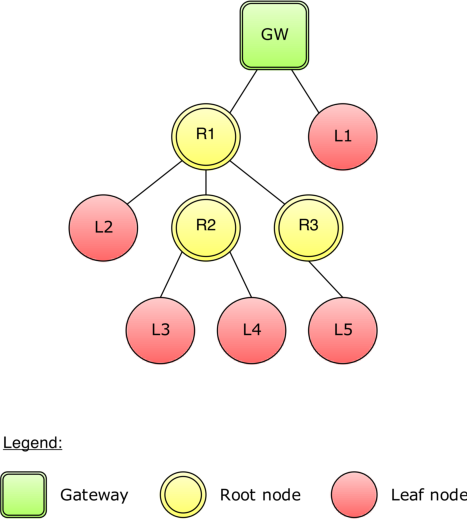
\includegraphics{img/network_topology.pdf}
	\end{center}
	\caption{\small \itshape{Network topology}}
	\label{img:network_topology}
\end{figure}

When joining the network new nodes must choose an existing root node as their
parent. Our implementation of the decision process is designed to maintain a balanced
tree structure, with minimum depth and to minimize packet-loss. The
most influential factor in the decision is the node's hop-count to the gateway.
By choosing the root node with the smallest hop-count we keep the tree depth at
a minimum. The second most influential factor is the node's signal strength.
Choosing the node with the greatest signal strength assures a lower
packet-loss rate. The third decision factor is the number of children the root
node already has. By associating with nodes that have the least number of
children we maintain the balance of the tree structure and the work load.

Activity in the network is cyclic. The time period with which actions are
repeated is called the \emph{network period}. For synchronization purposes it
is divided into time slots and each time slot is dedicated to a specific
communication. Slots must be long enough to accommodate two full-length
transmissions: one message and one acknowledgement. We must also take into
account clock drift. To do this we add a guard time to compensate for nodes
running too fast and a guard time to compensate for nodes running to slow.
These guard times are dependant on the network period and on the clock drift
rate, which is a constant given by the manufacturer. Because most transmissions
will be short, we place both guard spaces at the end of the slot to maximize
sleep times.

\begin{figure}[ht]
	\begin{center}
		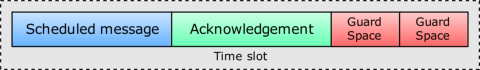
\includegraphics[width=\textwidth]{img/time_slot.pdf}
	\end{center}
	\caption{\small \itshape{Time slot overview}}
\end{figure}

No more than one node may be active in the network at a time, except for
contention periods. Although this approach is not efficient from a bandwidth
utilisation point of view, as nodes that are not in range of each other can be
active at the same time, we have chosen this approach to avoid the hidden and
exposed terminal problems\cite{jayasuriya2004hidden}. 

\section{Initialization and registering to the network}
\label{sec:initialization_and_registering_into_the_network}

After power-on all Sparrow nodes will first read their pre-programmed id from
the \mbox{EEPROM} memory and then attempt to register to a network. No
restrictions such as network address or parent id are imposed. As such, any
distribution of Sparrow nodes will eventually form a network under two
assumptions: all leaf nodes are within communication distance of at least one
root node and a path can be formed from any root node to the gateway.

There are two major approaches to registering to a network: the new node can
request registration information from the existing nodes (request method) or
the existing nodes can periodically advertise this information for new nodes
(advertisement method). 

\subsection{Request method}

The first method implies that any new node must broadcast a discovery message,
wait for responses, choose the best parent node from the offers received and
finally register to that node. With this method registration can be
unsuccessful for a number of reasons.

Firstly, there may be no root nodes within communication distance of the new
node. The most we can do in this situation is set a timeout and, if this
timeout is reached and no offer is received, place the node in a sleep state
and retry the procedure after a certain amount of time.

Secondly, there may be root nodes in range but none are awake or in the
listening state. This can be partially solved by prolonging root node listening
periods, albeit to the detriment of power consumption.

Thirdly, there may be root nodes in listening mode and in range but the
discovery message may be corrupted by an already scheduled transmission. The
possibility of this happening can be reduced by grouping transmissions within
the root node's listening period.

Fourthly, considering that the discovery message was
successfully received, the offer message may be corrupted because two nodes
attempt to respond at the same time. This means that a contention period must
precede any response, lengthening the registering node's listening window and
possibly requiring multiple attempts from the root nodes in order to
respond.

Lastly, considering that the discovery message was received and there was at
least one offer, the following message sequence, i.e. the actual registration
process, may be corrupted by a scheduled transmission or other phenomenon and
the process will have to be repeated. This may avoided through advanced
communication scheduling.

As can be seen, this method implies low costs for the registering nodes as they
must only transmit the discovery message and listen a relatively short time for
offers. Moreover they must pay this cost only once, during the registering process.
Root nodes however must listen for long periods of time which implies a high
power cost that must be payed for every network period. Furthermore, this method
does not scale well with the number of nodes in the network. The chances of the
discovery message interfering with a scheduled transmission increase with the
number of nodes in the network. The same applies if more nodes are attempting
to register at the same time. This means that as the network grows it will
become increasingly difficult for new nodes to join.

\subsection{Advertisement method}
\label{subsec:advertisement_method}

The second method involves all root nodes periodically transmitting a beacon,
or Router Advertisement, that contains all the information necessary to
register to the network. New nodes must listen for these messages and then
communicate with their chosen parent in order to register. This procedure also
has a number of issues that we must address.

Firstly, there may be no root nodes in range of the new node so, as with the
first method, the best we can do is to set a timeout and retry the registration
process.

Secondly, although there is at least one root node in range, the request may
interfere with a scheduled transmission. To avoid this, we reserve a
registration slot for each root node in which it listens for incoming requests
and in which no other communication is scheduled.

Thirdly, although the request may have been sent within the root
node's registration slot, it was corrupted by another node attempting to
register to the same root. This can be resolved by adding a contention slot
before the registration. A node must first listen for a random period of time
and then successfully transmit a message to the root node in the contention
period in order to begin the registration process.

Finally, there is no
guarantee that there will be a victor after the contention process. Sparrowv3
nodes have a 17 μs transition delay between listening and transmitting states
which means that if two nodes are offset by less than this they cannot avoid
each other and a collision will happen. This can be resolved by making
listening periods multiples of 17us or more, so that two nodes that choose 
different random listening periods cannot interfere with each other.

This method implies a longer listening period for registering nodes but this
cost must only be paid once. The cost for root nodes is relatively low as they
must only transmit the advertisement message and have two extra listening
slots. It also scales relatively well with the number of nodes in the network.
If all contentions have a winner then the mean waiting time scales
proportionally to the number of nodes attempting to register with a root node. 

\vspace{\baselineskip}

As the comparison shows, the advertisement method is the better choice for
Wireless Sensor Networks as the average cost of registration is lower and it
scales better with network growth. In our implementation new nodes do not
initially know the network period, so they must extract it from the first
Router Advertisement they receive. Then they wait one network period to collect
advertisements, choose the best root node available as their parent and set a
wake-up timer for the contention slot. In the contention phase the node chooses
a random listening period that is at most the full contention slot. If another
transmission is received, the node goes back to sleep and retries registering
in the next network period. If there is no other transmission, it sends a
registration request in which it specifies whether it is a root or leaf node.
Leaf nodes are allocated one transmission slot whereas root nodes are
implicitly allocated 16. If this request is received correctly by the root
node, i.e. a conflict has not occurred, the root node acknowledges the
registration and the new node transitions into normal operating mode.

\section{Leaf node operation}
\label{sec:leaf_node_operation}

The main focus of leaf node operation is low power consumption. They are only
active during the communication slot with their parent. In this slot they
transmit a message to their parent and wait for an acknowledgement message.
Then they synchronize their time source according to the information received
in the acknowledgment message. If the acknowledgement does not arrive, the
frame is considered lost but it is not retransmitted. If 10 transmissions is a
row fail then the parent node is considered to have gone off-line and the node
tries to re-register to the network. 

The SparrowLibrary allows the user to specify two additional activities. The
first is a function to be called after a frame is received. The second is a
function to be called before a frame is to be transmitted. Through these
functions the programmer may interact with the application frame buffer. For
the transmission callback the user must also specify how long before the
transmission window the function should be called. The programmer is
responsible for estimating the duration of the callback. If the estimation is
too short the transmission timeout will interrupt the function and its
execution will be resumed after the transmission is started. The function can
also be interrupted again when the acknowledge message is received.

\section{Root node operation}
\label{sec:root_node_operation}

The root nodes' responsibilities in the network are much more elaborate than
those of leaf nodes. Obviously, this comes with a higher duty cycle and power
consumption. 

Firstly, in the registration phase root nodes will be allocated 16 time slots
and they are responsible for allocating them to their children. In the case
that these slots become exhausted a root node can request another 16 time slots
from its parent. After registering, the root node will transmit one locally
generated message to its parent every network period and wait for an
acknowledgement. This frame is sent during the 13\textsuperscript{th} time slot
of this block. The 14\textsuperscript{th} and 15\textsuperscript{th} slots are
the contention and registration slots. Slots 1 through 12 are reserved for
receiving data from the node's children and transmitting this data forward. For
example, the data received from the node in slot 3 is sent forward towards the
gateway in slot 9. This way only one frame must be buffered, reducing the
node's memory usage. The 16\textsuperscript{th} slot is reserved for the Router
Advertisement.

\begin{figure}[ht]
	\begin{center}
		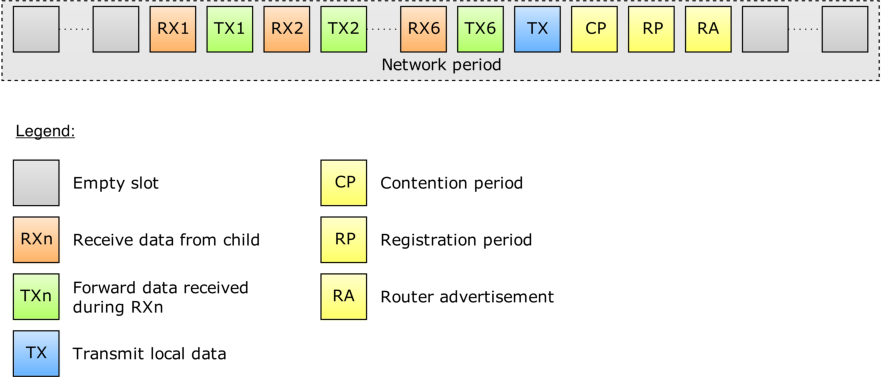
\includegraphics[width=\textwidth]{img/root_node_operation.pdf}
	\end{center}
	\caption{\small \itshape{Root node operation}}
\end{figure}

Secondly, the node must be able to allocate time slots for new nodes that wish
to join the network and existing root nodes that require more slots. In either
case time slots are allocated from the node's pool in descending order. There
are two moments when the node may be required to allocate new slots: during the
registration period and during the reception periods. In the registration slot
new nodes may requests to join the network and ask for one slot, if a leaf node
is registering, or 16 slots, if a root node is registering. In the reception
slots the sender node may include a request for more slots in the message, but
this request will only be taken into consideration after the contention period
so as to not hinder new nodes from joining the network. In either case, the
root node will accept the request if it has enough slots available and deny it
otherwise.  

Thirdly, root nodes must transmit Router Advertisements in order to allow new
nodes to join the network. The advertisement message contains the root node's
id, the network period and the number of free slots that the node has. The fact
that the advertisement is sent in the last time slot ensures that the number of
available slots will not change until the next contention period.

Fourthly, if during 10 consecutive reception periods no message is received
from the child in question, the root node will mark the slot as free and
advertise it as such.

Finally, it must provide its children with synchronization information. When a
scheduled message arrives from a child node the root node calculates the offset
between the moment when the frame was supposed to arrive and the actual arrival
time and includes this information it the acknowledgement message.

\section{Gateway operation}

The gateway becomes active after initialization and does not pass through the
registration phase.

It initially owns all time slots within the network period and allocates slots
to other nodes upon requests. After a slot is allocated to a node that node
becomes the slot's owner and can use it as described in sections
\ref{sec:leaf_node_operation} and \ref{sec:root_node_operation}. An example
slot allocation, for the network shown in figure \ref{img:network_topology} is
presented in figure \ref{img:slot_allocation}.

\begin{figure}[ht]
	\begin{center}
		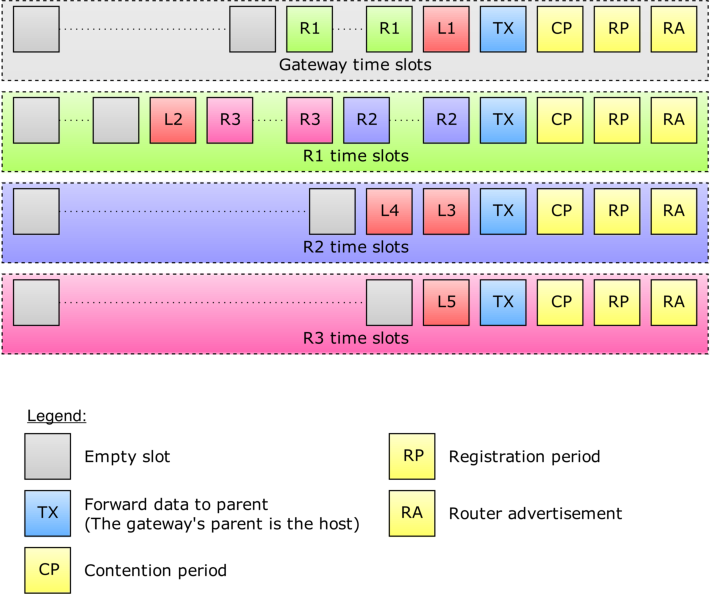
\includegraphics[width=\textwidth]{img/slot_allocation.pdf}
	\end{center}
	\caption{\small \itshape{Time slot allocation example}}
	\label{img:slot_allocation}
\end{figure}

It is also the only node to have the network period pre-programmed. As stated
in section \ref{sec:initialization_and_registering_into_the_network}, all other
nodes learn this information through Router Advertisements. As the gateway has
all the same functionality as a root node, it advertises its presence and nodes
register to the network through it. These nodes, if they are root nodes, send
advertisements and more distant nodes can now join the network.

The gateway's time source is the reference clock for the entire network. All
its children synchronize to its time. 

% ********** End of Sparrow protocol **********
